\graphicspath{{content/chapters/5_evaluation/figures/}}

\chapter{Evaluation}%
\label{chp:evaluation}
\rule{\textwidth}{1pt} \\[1ex]

\epigraph{\textit{``It is not the strongest of the species that survive, nor the most intelligent, but the one most responsive to change.''}}{\textbf{-- Charles Darwin}}

\section{Introduction}
\label{sec:5_introduction}
% Grazzi Sinjur Alla, Ahfirli Sinjur Alla, u Ismaghni Sinjur Alla. Grazzi Amen

\section{Hardware Setup}
\label{sec:5_hardware_setup}

All experiments involving deep learning models were conducted using two primary hardware configurations. Training was performed on systems equipped with an NVIDIA GeForce RTX 4070 and an RTX 4090 \gls{gpu}, both supporting \gls{cuda}-enabled acceleration. These setups were used across different experiments as needed, enabling parallel computation and helping to reduce training times significantly.


\section{Optimal Tiling Experiments}
\label{sec:5_tiling_exp}
% Glorja lil Missier, lil-Iben u lil- Ispirtu s-Santu, Kif kien fil bidu, issa u dejjem, ghal-dejjem. Amen. Grazzi Mulej
% all altitudes aggregated, since we require a detection model capable of generalising to different altitudes, definition of objects

%IMP Uncomment figures as you go along
To determine the most suitable tiling parameter for pre-processing the \gls{soda} dataset, a series of experiments were conducted. The objective was to identify an appropriate grid size for effective tiling. Although the authors in \cite{detect_litter} proposed a 5$\times$5 configuration, they offered no clear justification for selecting that specific size.
Tiling is applied in this context to increase the apparent size of small litter objects, which appear relatively diminished due to the high-altitude perspective (see Figure \ref{fig:tiling_examples}). As the grid becomes finer, these objects occupy a larger proportion of each tile. This can potentially improve detection accuracy. A larger grid size, therefore, appears beneficial in this respect.

However, increasing the grid size introduces new challenges. The most significant issue is the additional burden on processing and inference time. More tiles are produced, which in turn means more data needs to be handled during model evaluation. This added complexity can lead to slower performance if not carefully managed \cite{tiling}.
As such, choosing a grid size involves balancing two competing goals. One is to make small objects more detectable. The other objective is to prevent a significant rise in computational cost. As such, identifying an optimal balance between object visibility and processing efficiency requires further exploration.

In this study, an experiment was carried out to identify the optimal tiling grid size by measuring the rate of change in small object detection and the number of resulting images as the grid size varied. The first step involved establishing a classification scheme for object sizes. For this purpose, the definitions provided by the \gls{coco} dataset \cite{coco} were adopted, and are summarised below:

\begin{adjustwidth}{4em}{0pt} % Indent 2em from the left
\begin{description}
    \item[Small:] Objects occupying an area of less than $32 \times 32$ pixels.
    \item[Medium:] Objects with sizes ranging from $32 \times 32$ to $96 \times 96$ pixels.
    \item[Large:] Objects exceeding $96 \times 96$ pixels in area.
\end{description}
\end{adjustwidth}

With these definitions in place, the experiment proceeded by testing a range of grid sizes from 1 to 10. A grid size of 1 represents the original image with no tiling applied, while a grid size of 10 results in each image being divided into 100 tiles. For each configuration, the rate of change was recorded for small, medium, and large objects, as well as the total number of annotations and images.
A key consideration was the treatment of annotations that spanned tile boundaries. In such cases, these annotations were duplicated across the relevant tiles, leading to an expected increase in annotation count. This effect was deliberately preserved to reflect how tiling may influence the volume of training data. Each tile was also resized to 800 by 800 pixels to ensure consistency in size across all tiling configurations. This resizing was essential for maintaining uniform object scale during analysis, as 800 pixels was the chosen model input size throughout this study (refer to Subsection \ref{subsec:4_resizing}).

\begin{figure}[!ht]
  \centering
  \begin{tabular}{c}
    \includegraphics[width=0.9\textwidth]{optimal_tiling_experiment_results_line1.png} \\
    \small (a) \\
    \addlinespace[1em]
    \includegraphics[width=0.9\textwidth]{optimal_tiling_experiment_results_line2.png} \\
    \small (b) \\
  \end{tabular}
  \caption{Optimal tiling experiment results on the \gls{soda} dataset, illustrating the increase in the number of images and annotated objects as the grid size increases. (a) Results over the full altitude range (1--30 metres), and (b) results on a subset of altitudes (5--30 metres) from the \gls{soda} dataset.}
  \label{fig:optimal_tiling_line}
\end{figure}

Two separate experiments were conducted. The first included the full \gls{soda} dataset, covering altitudes from 1 metre to 30 metres. The second considered a subset with altitudes ranging from 5 metres to 30 metres. These configurations were selected to examine whether including very close-range images (such as those at 1 metre) would affect the optimal grid size. The ultimate objective is to develop a single detection model capable of operating effectively across various altitudes. The results of these experiments are presented in Figure~\ref{fig:optimal_tiling_line}.

The results of both experiments demonstrate that, as grid size increases, the number of images and annotations also increases. Conversely, the number of small objects decreases, while the count of medium and large objects rises. In the experiment covering all altitudes, the rate of change was more extreme, largely due to the presence of large objects captured at the 1-metre altitude. In contrast, the experiment excluding 1-metre data showed more gradual, consistent changes. Despite this difference, both experiments exhibited the expected trends based on the tiling behaviour.
However, these outcomes alone do not provide a direct conclusion regarding the optimal grid size. The goal remains to identify a configuration that reduces the proportion of small objects without introducing excessive computational overhead from processing a high number of tiles. To this end, the ratio of small objects to the number of generated tiles was examined across grid sizes, as shown in Figure \ref{fig:elbow_plot}.

\begin{figure}[!ht]
  \centering
  \begin{tabular}{c}
    \includegraphics[width=0.9\textwidth]{optimal_tiling_experiment_elbow_method1.png} \\
    \small (a) \\
    \addlinespace[1em]
    \includegraphics[width=0.9\textwidth]{optimal_tiling_experiment_elbow_method2.png} \\
    \small (b) \\
  \end{tabular}
  \caption{Ratio of small objects to the number of images plotted against tiling grid size, highlighting the observed elbow point in red. (a) Results over the full altitude range (1--30 metres), and (b) results on a subset of altitudes (5--30 metres) from the \gls{soda} dataset.}
  \label{fig:elbow_plot}
\end{figure}

To determine the optimal grid size, the elbow point \cite{elbow_point} method was applied. This approach involved calculating the first and second derivatives of the curve, identifying the point at which the rate of change begins to level off. The second derivative was particularly useful in locating the inflection point, where diminishing returns set in.
Interestingly, both experiments pointed to a 3$\times$3 grid as the optimal configuration. It is worth noting, however, that although the trends across both plots were similar, the ratio of small objects per tile was higher in the all-altitudes experiment. This suggests that including close-range imagery may influence the density of small object annotations.
As a result of this experiment, the tiling configuration used for dataset pre-processing in this study was set to a 3$\times$3 grid for the \gls{soda} dataset (refer to Subsection \ref{subsec:4_soda}), in line with the findings outlined above.

\section{Within-Dataset Evaluation}
\label{sec:5_within_dataset_exp}
% Grazzi Sinjur Alla, Ahfirli Sinjur Alla, u Ismaghni Sinjur Alla. Amen.

% N.B. Visual results and confusion matrix as well, explain different value of alpha, why they were chosen

To assess the proposed integration of the \gls{lupi} paradigm within object detection, litter detection was selected as one of the case studies. This task presents a particularly challenging scenario, largely due to the frequent presence of small objects, which considerably complicates the detection process. To examine the effectiveness of the proposed methodology under such conditions, a within-dataset evaluation was conducted using the \gls{soda} dataset.

The \gls{soda} dataset was purposefully chosen as the principal dataset for training \gls{uav}-based litter detection models. Its selection stems from its capacity to represent a diverse range of altitudes and litter types--characteristics not fully captured by the other available \gls{uav}-based litter datasets. The within-dataset evaluation comprised three core experiments: (i) binary litter detection using only the 1-metre altitude subset with no tiling; (ii) binary litter detection on the full \gls{soda} dataset, tiled using a 3$\times$3 grid and covering all altitudes; and (iii) multi-label litter detection using the same 3$\times$3 tiled version across all altitudes. Each of these configurations was chosen for a specific purpose: the first experiment targets detection at close range, the second expands the scope across variable altitudes, and the third introduces additional classification complexity by extending from binary to multi-label tasks, distinguishing between various litter types and the background.

For each of these experiments, the five object detection architectures detailed in Section \ref{sec:4_distillation_architectures} were trained: Faster \gls{rcnn}, \gls{ssd}, RetinaNet, SSDLite, and \gls{fcos}. Each architecture produced a baseline model, a teacher model, and four student models trained with varying levels of teacher guidance. Consequently, 30 distinct models were trained for each experiment.

The central objective was to determine whether student models trained using the \gls{lupi} framework, with access to privileged training signals, could outperform their respective baselines, which were trained using only standard input data. For each architecture, a teacher model was first trained, followed by the training of student models using five distinct \gls{alpha} values: 0, 0.25, 0.5, 0.75, and 1. These values match those used in related work in \gls{lupi} \cite{lab2wild}. An $\alpha$ of 0 represents the baseline, where the student is trained without any guidance from the teacher, while $\alpha = 1$ reflects full reliance on the teacher’s output during training. The intermediate values allowed a controlled study of how varying degrees of teacher influence affected model performance.


Importantly, this study did not involve cross-architecture distillation. In other words, teacher models were used only to train student models of the same architecture. This approach was adopted to avoid the added complexity of aligning latent feature representations between different model types, which would have required additional mechanisms and exceeded the scope of this work.

All models were trained using the designated training subsets, while validation and testing were carried out on their respective data partitions. The evaluation followed the detection metrics outlined in Section \ref{sec:4_metrics}, providing a consistent basis for comparison. A uniform pre-processing pipeline and identical training configurations were applied across all models, ensuring fairness in evaluation. Given the diverse range of detection architectures and the controlled experimental setup, the resulting outcomes offer a reliable and concrete basis for assessing the influence of \gls{lupi} in object detection.


\subsection{Binary Litter Detection on the SODA Dataset at 1-Metre Altitude}
\label{subsec:5_soda01m_dataset_exp}
% Glorja lil Missier lil Iben u lil Ispirtu s-Santu, Grazzi. Amen

The first experiment aimed to assess the benefits of using the \gls{lupi} framework for close-range litter detection. To this end, a subset of the \gls{soda} dataset at a 1-metre altitude was selected, consisting of 452 images. These images were divided into 316 for training, 46 for validation, and 90 for testing. In this experiment, detection models were trained to classify all litter into a single category, distinguishing between litter (foreground) and background.

The results of this experiment, comparing the baseline model with the best student model across all five selected detection architectures, are presented in Figure \ref{fig:soda01m_bar}. In all architectures, the student model outperformed the baseline, showing a notable improvement in detection accuracy, particularly in the challenging \gls{map}@50–95 metric. Additionally, improvements were seen in other key detection metrics, including precision, recall, and F1 score. Among the models, the RetinaNet student achieved the highest performance, followed by the Faster \gls{rcnn} and \gls{fcos} student models. Across all metrics, the student models demonstrated an accuracy improvement ranging from 0.5 to 0.15. Interestingly, when comparing the baseline models with the student models, RetinaNet and \gls{ssd} showed the highest improvements in detection accuracy, with the student models outperforming their baseline counterparts. The other architecture types, such as Faster \gls{rcnn} and \gls{fcos}, also saw improvements, though the performance boosts were somewhat smaller in comparison to those of RetinaNet and \gls{ssd}.

\begin{figure}[!ht]
    \centering
    \includegraphics[width=1\textwidth]{SODA 01m Dataset (Single-label).png}
    \caption{Comparison between the baseline and the best-performing student models across key detection metrics on the \gls{soda} dataset at a 1-metre altitude for binary litter detection.}
    \label{fig:soda01m_bar}
\end{figure}

While RetinaNet, \gls{fcos}, and Faster \gls{rcnn} delivered the best results in this experiment, which can be attributed largely to their complex architectures and the use of the ResNet-\gls{fpn} backbone, notable improvements were also observed with the \gls{ssd} and SSDLite architectures. This suggests that the \gls{lupi} method can improve litter detection performance at close range, even in complex environments with backgrounds such as rocks and plants. The results indicate that, regardless of the architecture, \gls{lupi} significantly improves detection accuracy, confirming its efficacy for binary detection tasks at close proximity.

In addition to the comparison between the baseline and student models, a further analysis was conducted to evaluate the performance of the different teacher models, using the same evaluation metrics and experimental setup. The results are summarised in Table~\ref{tab:teacher_model_metrics_soda01m}, which presents the detection accuracy achieved by each teacher model architecture. It can be observed that Faster \gls{rcnn}, \gls{fcos}, and RetinaNet stood out as the highest-performing teacher models. Most of their detection metrics approached 1.0, suggesting near-ideal detection performance across the evaluated scenes. 
% These results highlight the informative nature of these teacher networks, especially in supporting the \gls{lupi} training paradigm.

\begin{table}[!ht]
    \centering
    \begin{adjustbox}{max width=\textwidth}
    \renewcommand{\arraystretch}{1.5}
    \begin{tabular}{|l|c|c|c|c|c|c|c|c|c|}
        \hline%\toprule
        \textbf{Model} & \textbf{mAP@50--95} & \textbf{mAP@50} & \textbf{mAP@75} & \textbf{mAR@1} & \textbf{mAR@10} & \textbf{mAR@100} & \textbf{Precision} & \textbf{Recall} & \textbf{F1 Score} \\ \hline \hline
        \textbf{RetinaNet} & 0.94 & 0.98 & 0.96 & 0.63 & 0.96 & 0.96 & 0.93 & 0.99 & 0.96 \\\hline
        \textbf{FCOS} & \textbf{0.96} & 0.98 & 0.97 & 0.63 & 0.97 & 0.97 & 0.81 & 0.99 & 0.89 \\\hline
        \textbf{Faster R-CNN} & \textbf{0.96} & \textbf{0.99} & \textbf{0.98} & \textbf{0.63} & \textbf{0.98} & \textbf{0.98} & \textbf{0.99} & \textbf{0.99} & \textbf{0.99} \\\hline
        \textbf{SSD} & 0.78 & 0.96 & 0.94 & 0.54 & 0.81 & 0.81 & 0.65 & 0.99 & 0.79 \\\hline
        \textbf{SSDLite} & 0.61 & 0.73 & 0.72 & 0.48 & 0.63 & 0.63 & 0.02 & 0.99 & 0.03 \\
        \hline%\bottomrule
    \end{tabular}
    \renewcommand{\arraystretch}{1}
    \end{adjustbox}
    \caption{Comparison of teacher model performance across key detection metrics, trained on the \gls{soda} dataset at a 1-metre altitude for binary litter detection.}
    \label{tab:teacher_model_metrics_soda01m}
\end{table}

On the other hand, the \gls{ssd} and SSDLite teacher models, while still achieving reasonable scores, demonstrated noticeably lower accuracy. Even when trained with privileged information, these architectures did not attain the same level of conceptual understanding, indicating limitations in adapting to this particular detection task. Combined with the student model results in Figure~\ref{fig:soda01m_bar}, this suggests that these architectures may be less suited to scenarios requiring high sensitivity to fine-grained object features.

Interestingly, while Faster \gls{rcnn} proved to be the top-performing teacher model, it was not associated with the best-performing student. That distinction went to the RetinaNet student model. Given that both architectures share a similar ResNet-\gls{fpn} backbone and were distilled at equivalent feature extraction stages, this outcome suggests that RetinaNet may be structurally more compatible with learning using privileged information in this context.

Across all teacher models, recall was generally high, while precision tended to be lower. This implies that the teacher models were primarily geared toward minimising \gls{fn}, reinforcing their utility in guiding student models to identify more instances, albeit sometimes at the expense of \gls{fp}.

While the results clearly show that \gls{lupi} improves detection accuracy in this particular experiment, it is also important to acknowledge that this improvement does not come without cost. Training within the \gls{lupi} framework requires an additional training phase, wherein a teacher model must be trained before the student. Moreover, each model must process privileged inputs during training, resulting in larger tensors and increased computational demands, despite only minor adjustments to the teacher architecture and none to the student.

To examine the impact of these changes on training duration, Figure~\ref{fig:soda01m_training_time} presents a comparison of training times across all models involved in this experiment. As shown in the figure, both student and teacher models required substantially more time to train than the baseline models. This increase is due in part to the two-stage nature of the training process and, for student models specifically, the added computation needed to process the teacher’s outputs and compute the distillation loss. The time taken by the teacher during inference directly contributes to the student’s overall training time.

\begin{figure}[!ht]
    \centering
    \includegraphics[width=1\textwidth]{training_times_soda_01m_dataset_binary_detection.png}
    \caption{Comparison of model training times on the \gls{soda} dataset at a 1-metre altitude for binary litter detection.}
    \label{fig:soda01m_training_time}
\end{figure}

In terms of model-specific performance, \gls{fcos} and SSDLite exhibited the shortest training durations, whereas RetinaNet and Faster \gls{rcnn} incurred the highest training times, especially under the \gls{lupi} setup. Notably, teacher models consistently recorded the longest training durations across all architectures.

Despite the increase in training time, a comparison of model size and parameter count between the baseline and student models, as shown in Table~\ref{tab:model_configs_soda01m}, shows that they remain identical across all architectures. This suggests that student models benefit from improved detection accuracy through \gls{lupi} without adding any cost in terms of model size or computational demands during inference. In contrast to many modern detection models that require larger storage and are computationally intensive at deployment \cite{detr, rt-detr, rt-detrv2, rf-detr}, the student models preserve the compactness of their baseline versions.

\begin{table}[!ht]
    \centering
    \begin{tabular}{llcc}
        \toprule
        \textbf{Model Configuration} & \textbf{Type} & \textbf{Size (MB)} & \textbf{Parameters (M)} \\
        \midrule
        \multirow{5}{*}{\textbf{Baseline}} 
            & RetinaNet   & 122.72 & 32.17 \\
            & FCOS        & 122.32 & 32.06 \\
            & Faster R-CNN & 157.54 & 41.30 \\
            & SSD         & 90.58  & 23.75 \\
            & SSDLite     & 8.42   & 2.21 \\
        \midrule
        \multirow{5}{*}{\textbf{Student}} 
            & RetinaNet   & 122.72 & 32.17 \\
            & FCOS        & 122.32 & 32.06 \\
            & Faster R-CNN & 157.54 & 41.30 \\
            & SSD         & 90.58  & 23.75 \\
            & SSDLite     & 8.42   & 2.21 \\
        \bottomrule
    \end{tabular}
    \caption{Comparison of model configurations for trained baseline and student models on the \gls{soda} dataset at a 1-metre altitude for binary litter detection, including model type, size in megabytes, and number of parameters (in millions).}
    \label{tab:model_configs_soda01m}
\end{table}

It is also important to point out that Faster \gls{rcnn}, \gls{fcos}, and RetinaNet occupy more memory overall, as they rely on larger architectural designs. On the other hand, \gls{ssd} and SSDLite remain comparatively lightweight. Even so, the main observation remains clear. In the context of \gls{uav}-based binary litter detection, where lightweight architectures are essential due to hardware limitations, \gls{lupi} enables improved detection accuracy without increasing model size. This makes it a practical solution for situations where both storage and computational efficiency are important.

\subsection{Binary Litter Detection on the SODA Dataset Across All Altitudes}
\label{subsec:5_soda_tiled_single_dataset_exp}
% Glorja lil Missier, lil Iben u lil Ispirtu s-Santu. Amen

The second experiment aimed to build upon the context of the first by further exploring the benefits of using the \gls{lupi} framework for litter detection at higher altitudes, addressing the challenges posed by more complex detection scenarios. To this end, the entire \gls{soda} dataset was tiled in a 3$\times$3 configuration at all altitudes to reflect a more complex, real-world scenario for \gls{uav}-based litter detection. This dataset included 7,461 images, with 5,238 allocated for training, 765 for validation, and 1,458 for testing. In this experiment, detection models were trained to classify all litter into a single category, focusing on distinguishing small litter from variable and challenging backgrounds.

The results of this experiment, comparing the baseline model with the best-performing student model across all five selected detection architectures, are presented in Figure~\ref{fig:soda_tiled_single_bar}. In most cases, the student models performed better than their baseline counterparts, showing noticeable gains in detection accuracy, particularly in the more demanding \gls{map}@50–95 metric. However, the \gls{ssd} and SSDLite architectures exhibited little to no improvement.
Compared to the earlier experiment shown in Figure~\ref{fig:soda01m_bar}, the results here reflect a tougher detection setting, which generally led to lower overall performance. Even so, models trained with the \gls{lupi} framework still showed clear advantages. Notably, improvements were also observed in precision, recall, and F1 score metrics.

\begin{figure}[!ht]
    \centering
    \includegraphics[width=1\textwidth]{SODA Dataset (Tiled Binary Detection).png}
    \caption{Comparison between the baseline and best-performing student models across key detection metrics on the 3$\times$3 tiled \gls{soda} dataset across all altitudes for binary litter detection.}
    \label{fig:soda_tiled_single_bar}
\end{figure}

Among all models, the student version of Faster \gls{rcnn} delivered the best overall results, followed by \gls{fcos} and RetinaNet. This marks a shift from the previous experiment, where RetinaNet had achieved the highest scores. The performance of Faster \gls{rcnn} suggests that its two-stage architecture may be better suited to the demands of this task than the one-stage approaches. Furthermore, the student models outperformed their baseline counterparts across all evaluated metrics, with accuracy improvements ranging from 0.1 to 0.11. \gls{fcos} and Faster \gls{rcnn} recorded the most noticeable performance boosts compared to their baselines. RetinaNet and SSDLite also benefitted, though to a lesser degree. For \gls{ssd}, the improvement was limited, appearing only in the \gls{map}@75 metric.

Moreover, the findings further support the selection of Faster \gls{rcnn}, \gls{fcos}, and RetinaNet as more effective detection architectures in this context, especially when compared to the lighter alternatives, owing to their structural complexity and performance consistency.
In addition to this comparison, a further analysis was carried out to assess the efficacy of different teacher models, following a similar approach to the previous experiment. The outcomes, presented in Table~\ref{tab:teacher_model_metrics_soda_tiled_single}, detail the detection accuracy attained by each teacher architecture. Once again, Faster \gls{rcnn}, \gls{fcos}, and RetinaNet emerged as the top performers, with several of their metrics approaching ideal values, though with slight reductions in some areas. These results indicate that, despite the increased scene complexity, these models continue to demonstrate high detection accuracy.

\begin{table}[!ht]
    \centering
    \begin{adjustbox}{max width=\textwidth}
    \renewcommand{\arraystretch}{1.5}
    \begin{tabular}{|l|c|c|c|c|c|c|c|c|c|}
        \hline
        \textbf{Model} & \textbf{mAP@50--95} & \textbf{mAP@50} & \textbf{mAP@75} & \textbf{mAR@1} & \textbf{mAR@10} & \textbf{mAR@100} & \textbf{Precision} & \textbf{Recall} & \textbf{F1 Score} \\ \hline \hline
        \textbf{RetinaNet} & 0.90 & 0.95 & 0.94 & 0.34 & 0.83 & 0.91 & 0.41 & 0.98 & 0.58 \\\hline
        \textbf{FCOS} & 0.89 & 0.94 & 0.93 & 0.34 & 0.82 & 0.90 & \textbf{0.97} & 0.96 & 0.96 \\\hline
        \textbf{Faster R-CNN} & \textbf{0.96} & \textbf{0.99} & \textbf{0.98} & \textbf{0.35} & \textbf{0.87} & \textbf{0.97} & 0.96 & \textbf{0.99} & \textbf{0.98} \\\hline
        \textbf{SSD} & 0.49 & 0.62 & 0.59 & 0.27 & 0.51 & 0.51 & 0.16 & 0.97 & 0.27 \\\hline
        \textbf{SSDLite} & 0.18 & 0.23 & 0.19 & 0.17 & 0.19 & 0.19 & 0.00 & 0.79 & 0.01 \\
        \hline
    \end{tabular}
    \renewcommand{\arraystretch}{1}
    \end{adjustbox}
    \caption{Comparison of teacher model performance across key detection metrics, trained on the 3$\times$3 tiled \gls{soda} dataset across all altitudes for binary litter detection.}
    \label{tab:teacher_model_metrics_soda_tiled_single}
\end{table}

The \gls{ssd} and SSDLite teacher models, although yielding acceptable results, showed a marked decline in detection accuracy when compared to the other models. This drop was especially apparent when examining performance across key metrics, highlighting a distinct limitation in their ability to generalise under the demands of this task. Even with access to privileged information, these models failed to match the conceptual accuracy achieved by the more capable architectures, suggesting they are less well-suited to scenarios requiring heightened sensitivity to fine-grained object features.

In contrast to the first experiment conducted at 1 metre altitude, Faster \gls{rcnn} emerged as the most effective teacher and student model in this multi-altitude experiment. RetinaNet, which incorporates focal loss to address class imbalance between foreground and background, underperformed relative to both Faster \gls{rcnn} and \gls{fcos}, with some detection metrics showing a gap of 0.1 or more in terms of the models outlined in Figure \ref{fig:soda_tiled_single_bar}. This suggests that RetinaNet may not be ideally suited for detecting litter in scenes characterised by visually complex and variable backgrounds. \gls{fcos}, leveraging centreness loss to improve spatial accuracy, delivered results on par with Faster \gls{rcnn} across both baseline and student models, reinforcing its reliability under these conditions.

Notably, the consistent use of the ResNet-\gls{fpn} backbone across Faster \gls{rcnn}, \gls{fcos}, and RetinaNet likely contributed to their relative success. The \gls{fpn}’s capacity for multi-scale object detection aligns well with the demands of \gls{uav}-based litter detection at varying altitudes. This architectural feature appears to bolster compatibility with learning via privileged information.

Across the teacher models, recall remained consistently high, while precision tended to be lower. Once again, this suggests that the models were primarily geared toward reducing \gls{fn}, which is generally beneficial in domains where missing detections is costly. However, in the context of litter detection, this emphasis may be less appropriate, as an increase in \gls{fp} can also undermine model reliability.


%--


% \begin{figure}[!ht]
%     \centering
%     \includegraphics[width=1\textwidth]{training_times_soda_dataset_tiled_binary_detection.png}
%     \caption{Comparison of model training times on the 3$\times$3 tiled \gls{soda} dataset across all altitudes for binary litter detection.}
%     \label{fig:soda_tiled_single_training_time}
% \end{figure}

% \begin{table}[!ht]
%     \centering
%     \begin{tabular}{llcc}
%         \toprule
%         \textbf{Model Configuration} & \textbf{Type} & \textbf{Size (MB)} & \textbf{Parameters (M)} \\
%         \midrule
%         \multirow{5}{*}{\textbf{Baseline}} 
%             & RetinaNet     & 122.72 & 32.17 \\
%             & FCOS          & 122.32 & 32.06 \\
%             & Faster R-CNN  & 157.54 & 41.30 \\
%             & SSD           & 90.58  & 23.75 \\
%             & SSDLite       & 8.42   & 2.21 \\
%         \midrule
%         \multirow{5}{*}{\textbf{Student}} 
%             & RetinaNet     & 122.72 & 32.17 \\
%             & FCOS          & 122.32 & 32.06 \\
%             & Faster R-CNN  & 157.54 & 41.30 \\
%             & SSD           & 90.58  & 23.75 \\
%             & SSDLite       & 8.42   & 2.21 \\
%         \bottomrule
%     \end{tabular}
%     \caption{Comparison of model configurations for trained baseline and student models on the 3$\times$3 tiled \gls{soda} dataset across all altitudes for binary litter detection, including model type, size in megabytes, and number of parameters (in millions).}
%     \label{tab:model_configs_soda_tiled_single}
% \end{table}


\subsection{Multi-label Litter Detection on the SODA Dataset Across All Altitudes}
\label{subsec:5_soda_tiled_multi_dataset_exp}

% \begin{figure}[!ht]
%     \centering
%     \includegraphics[width=1\textwidth]{SODA Dataset (Tiled Multi-label Detection).png}
%     \caption{Comparison between the baseline and best-performing student models across key detection metrics on the 3$\times$3 tiled \gls{soda} dataset across all altitudes for multi-label litter detection.}
%     \label{fig:soda_tiled_multi_bar}
% \end{figure}

% \begin{table}[!ht]
%     \centering
%     \begin{adjustbox}{max width=\textwidth}
%     \renewcommand{\arraystretch}{1.5}
%     \begin{tabular}{|l|c|c|c|c|c|c|c|c|c|}
%         \hline
%         \textbf{Model} & \textbf{mAP@50--95} & \textbf{mAP@50} & \textbf{mAP@75} & \textbf{mAR@1} & \textbf{mAR@10} & \textbf{mAR@100} & \textbf{Precision} & \textbf{Recall} & \textbf{F1 Score} \\ \hline \hline
%         \textbf{RetinaNet} & 0.88 & 0.92 & 0.91 & 0.66 & 0.89 & 0.89 & 0.76 & 0.97 & 0.85 \\\hline
%         \textbf{FCOS} & 0.91 & 0.95 & 0.94 & 0.68 & 0.92 & 0.92 & 0.91 & 0.97 & 0.94 \\\hline
%         \textbf{Faster R-CNN} & \textbf{0.95} & \textbf{0.99} & \textbf{0.98} & \textbf{0.70} & \textbf{0.96} & \textbf{0.96} & \textbf{0.96} & \textbf{0.99} & \textbf{0.97} \\\hline
%         \textbf{SSD} & 0.36 & 0.49 & 0.45 & 0.33 & 0.41 & 0.41 & 0.59 & 0.76 & 0.63 \\\hline
%         \textbf{SSDLite} & 0.11 & 0.13 & 0.13 & 0.13 & 0.13 & 0.13 & 0.00 & 0.37 & 0.01 \\
%         \hline
%     \end{tabular}
%     \renewcommand{\arraystretch}{1}
%     \end{adjustbox}
%     \caption{Comparison of teacher model performance across key detection metrics, trained on the 3$\times$3 tiled \gls{soda} dataset across all altitudes for multi-label litter detection.}
%     \label{tab:teacher_model_metrics_soda_tiled_multi}
% \end{table}


% \begin{figure}[!ht]
%     \centering
%     \includegraphics[width=1\textwidth]{map_all_classes_soda_multi.png}
%     \caption{Comparison between the baseline and best-performing student models based on mean average precision by class on the 3$\times$3 tiled \gls{soda} dataset across all altitudes for multi-label litter detection.}
%     \label{fig:soda_tiled_multi_per_class}
% \end{figure}

% \begin{figure}[!ht]
%   \centering
%   \begin{tabular}{cc}
%     \includegraphics[width=0.48\textwidth]{cm1.png} &
%     \includegraphics[width=0.48\textwidth]{cm2.png} \\
%     \small (a) & \small (b) \\
%   \end{tabular}
%   \caption{Normalised confusion matrices on the 3$\times$3 tiled \gls{soda} dataset across all altitudes for multi-label litter detection, using the best-performing models of the same architecture: (a) baseline, (b) student.}
%   \label{fig:cm_soda}
% \end{figure}

% \begin{figure}[!ht]
%     \centering
%     \includegraphics[width=1\textwidth]{training_times_soda_dataset_tiled_multi_label_detection.png}
%     \caption{Comparison of model training times on 3$\times$3 tiled \gls{soda} dataset across all altitudes for multi-label litter detection.}
%     \label{fig:soda_tiled_multi_training_time}
% \end{figure}

% \begin{table}[!ht]
%     \centering
%     \begin{tabular}{llcc}
%         \toprule
%         \textbf{Model Configuration} & \textbf{Type} & \textbf{Size (MB)} & \textbf{Parameters (M)} \\
%         \midrule
%         \multirow{5}{*}{\textbf{Baseline}} 
%             & RetinaNet     & 123.11 & 32.27 \\
%             & FCOS          & 122.36 & 32.08 \\
%             & Faster R-CNN  & 157.64 & 41.32 \\
%             & SSD           & 93.13  & 24.41 \\
%             & SSDLite       & 8.68   & 2.28 \\
%         \midrule
%         \multirow{5}{*}{\textbf{Student}} 
%             & RetinaNet     & 123.11 & 32.27 \\
%             & FCOS          & 122.36 & 32.08 \\
%             & Faster R-CNN  & 157.64 & 41.32 \\
%             & SSD           & 93.13  & 24.41 \\
%             & SSDLite       & 8.68   & 2.28 \\
%         \bottomrule
%     \end{tabular}
%     \caption{Comparison of model configurations for trained baseline and student models on the 3$\times$3 tiled \gls{soda} dataset across all altitudes for multi-label litter detection, including model type, size in megabytes, and number of parameters (in millions).}
%     \label{tab:model_configs_soda_tiled_multi}
% \end{table}


\subsection{Alpha Parameter Experiment}
\label{subsec:5_alpha_exp}

% \begin{figure}[!ht]
%     \centering
%     \includegraphics[width=1\textwidth]{ablation_study_soda_01m.png}
%     \caption{Assessing the impact of the alpha (\gls{alpha}) parameter on student model performance, trained and evaluated on the \gls{soda} dataset at a 1-metre altitude for binary litter detection.}
%     \label{fig:ablation_soda01m}
% \end{figure}

% \begin{figure}[!ht]
%     \centering
%     \includegraphics[width=1\textwidth]{ablation_study.png}
%     \caption{Assessing the impact of the alpha (\gls{alpha}) parameter on student model performance, trained and evaluated on the 3$\times$3 tiled \gls{soda} dataset across all altitudes for multi-label litter detection.}
%     \label{fig:ablation_soda_tiled_multi}
% \end{figure}

\section{Cross-Dataset Evaluation}
\label{sec:5_cross_dataset_exp}

\subsection{Binary Litter Detection on the BDW Dataset}
\label{subsec:5_bdw_exp}

% \begin{figure}[!ht]
%     \centering
%     \includegraphics[width=1\textwidth]{BDW Dataset (Tested on Models Trained on SODA 01m Binary Detection).png}
%     \caption{Comparison of baseline and best-performing student models on key detection metrics using the \gls{bdw} dataset. The evaluated models were trained on the \gls{soda} dataset captured at 1-metre altitude for binary litter detection.}
%     \label{fig:bdw_bar}
% \end{figure}

\subsection{Binary Litter Detection on the UAVVaste Dataset}
\label{subsec:5_uavvaste_exp}

% \begin{figure}[!ht]
%     \centering
%     \includegraphics[width=1\textwidth]{UAVVaste Dataset (Tested on Models Trained on SODA Tiled Binary Detection).png}
%     \caption{Comparison of baseline and best-performing student models on key detection metrics using the UAVVaste dataset. The evaluated models were trained on the 3$\times$3 tiled \gls{soda} dataset across all altitudes for binary litter detection.}
%     \label{fig:uavvaste_bar}
% \end{figure}

\section{Pascal VOC 2012 Evaluation}
\label{sec:5_pascal_voc_dataset_exp}

% \begin{figure}[!ht]
%     \centering
%     \includegraphics[width=1\textwidth]{Pascal VOC 2012 Dataset (Multi-label Detection for 20 Classes) .png}
%     \caption{Comparison between the baseline and best-performing student models across key detection metrics on the Pascal VOC 2012 dataset for multi-label detection of 20 object classes.}
%     \label{fig:pascal_voc_bar}
% \end{figure}

% \begin{figure}[!ht]
%     \centering
%     \includegraphics[width=1\textwidth]{map_all_classes_pascal_voc_no_text.png}
%     \caption{Comparison between the baseline and best-performing student models based on mean average precision by class on the Pascal VOC 2012 dataset for multi-label detection of 20 object classes.}
%     \label{fig:pascal_voc_per_class}
% \end{figure}

% \begin{table}[!ht]
%     \centering
%     \begin{adjustbox}{max width=\textwidth}
%     \renewcommand{\arraystretch}{1.5}
%     \begin{tabular}{|l|c|c|c|c|c|c|c|c|c|}
%         \hline
%         \textbf{Model} & \textbf{mAP@50--95} & \textbf{mAP@50} & \textbf{mAP@75} & \textbf{mAR@1} & \textbf{mAR@10} & \textbf{mAR@100} & \textbf{Precision} & \textbf{Recall} & \textbf{F1 Score} \\ \hline \hline
%         \textbf{RetinaNet} & 0.77 & 0.86 & 0.79 & 0.60 & 0.81 & 0.81 & 0.26 & 0.90 & 0.38 \\\hline
%         \textbf{FCOS} & \textbf{0.80} & 0.88 & \textbf{0.82} & \textbf{0.61} & \textbf{0.84} & \textbf{0.84} & 0.43 & \textbf{0.91} & 0.56 \\\hline
%         \textbf{Faster R-CNN} & 0.77 & \textbf{0.91} & \textbf{0.82} & 0.59 & 0.82 & 0.82 & \textbf{0.56} & \textbf{0.91} & \textbf{0.68} \\\hline
%         \textbf{SSD} & 0.42 & 0.56 & 0.49 & 0.41 & 0.48 & 0.48 & 0.25 & 0.69 & 0.36 \\\hline
%         \textbf{SSDLite} & 0.49 & 0.61 & 0.54 & 0.46 & 0.55 & 0.55 & 0.04 & 0.79 & 0.07 \\
%         \hline
%     \end{tabular}
%     \renewcommand{\arraystretch}{1}
%     \end{adjustbox}
%     \caption{Comparison of teacher model performance across key detection metrics, trained on the Pascal VOC 2012 dataset for multi-label detection of 20 object classes.}
%     \label{tab:teacher_model_metrics_pascal_voc}
% \end{table}


% \begin{figure}[!ht]
%     \centering
%     \includegraphics[width=1\textwidth]{training_times_pascal_voc_2012_dataset_multi_label_detection_for_20_classes.png}
%     \caption{Comparison of model training times on the Pascal VOC 2012 dataset for multi-label detection of 20 object classes.}
%     \label{fig:pascal_voc_training_time}
% \end{figure}

% \begin{figure}[!ht]
%   \centering
%   \begin{tabular}{c}
%     \includegraphics[width=0.7\textwidth]{cm3.png} \\
%     \small (a) \\
%     \addlinespace[1em]
%     \includegraphics[width=0.7\textwidth]{cm4.png} \\
%      \small (b) \\
%   \end{tabular}
%   \caption{Normalised confusion matrices on the Pascal VOC 2012 dataset for multi-label detection of 20 object classes, using the best-performing models of the same architecture: (a) baseline, (b) student.}
%   \label{fig:cm_pascal_voc}
% \end{figure}

% \begin{table}[!ht]
%     \centering
%     \begin{tabular}{llcc}
%         \toprule
%         \textbf{Model Configuration} & \textbf{Type} & \textbf{Size (MB)} & \textbf{Parameters (M)} \\
%         \midrule
%         \multirow{5}{*}{\textbf{Baseline}} 
%             & RetinaNet     & 124.22 & 32.56 \\
%             & FCOS          & 122.48 & 32.11 \\
%             & Faster R-CNN  & 157.92 & 41.40 \\
%             & SSD           & 100.27 & 26.29 \\
%             & SSDLite       & 9.42   & 2.47 \\
%         \midrule
%         \multirow{5}{*}{\textbf{Student}} 
%             & RetinaNet     & 124.22 & 32.56 \\
%             & FCOS          & 122.48 & 32.11 \\
%             & Faster R-CNN  & 157.92 & 41.40 \\
%             & SSD           & 100.27 & 26.29 \\
%             & SSDLite       & 9.42   & 2.47 \\
%         \bottomrule
%     \end{tabular}
%     \caption{Comparison of model configurations for trained baseline and student models on the Pascal VOC 2012 dataset for multi-label object detection, including model type, size in megabytes, and number of parameters (in millions).}
%     \label{tab:model_configs_pascal_voc}
% \end{table}


\section{Comparison of Visual Results and Model Interpretability}
\label{sec:5_interpretability}

% \begin{figure}[ht]
%   \centering
%   \begin{tabular}{cc}
%     \includegraphics[width=0.47\textwidth]{visual1.jpg} &
%     \includegraphics[width=0.47\textwidth]{visual2.jpg} \\
%     \small (a) & \small (b) \\
%     \addlinespace[1em]
%     \includegraphics[width=0.47\textwidth]{visual3.jpg} &
%     \includegraphics[width=0.47\textwidth]{visual4.jpg} \\
%     \small (c) & \small (d) \\
%   \end{tabular}
%   \caption{Comparison of predictions from the best-performing detection model trained on the \gls{soda} dataset. (a) and (c) show baseline model outputs, while (b) and (d) illustrate predictions from the corresponding student model.}
%   \label{fig:visuals_soda}
% \end{figure}

% \begin{figure}[ht]
%   \centering
%   \begin{tabular}{cc}
%     \includegraphics[width=0.47\textwidth]{visual5.jpg} &
%     \includegraphics[width=0.47\textwidth]{visual6.jpg} \\
%     \small (a) & \small (b) \\
%     \addlinespace[1em]
%     \includegraphics[width=0.47\textwidth]{visual7.jpg} &
%     \includegraphics[width=0.47\textwidth]{visual8.jpg} \\
%     \small (c) & \small (d) \\
%   \end{tabular}
%   \caption{Comparison of predictions from the best-performing detection model trained on the Pascal \gls{voc} 2012 dataset. (a) and (c) show baseline model outputs, while (b) and (d) illustrate predictions from the corresponding student model.}
%   \label{fig:visuals_pascal_voc}
% \end{figure}

% Grad CAM citations
% \begin{figure}[!ht]
%     \centering
%     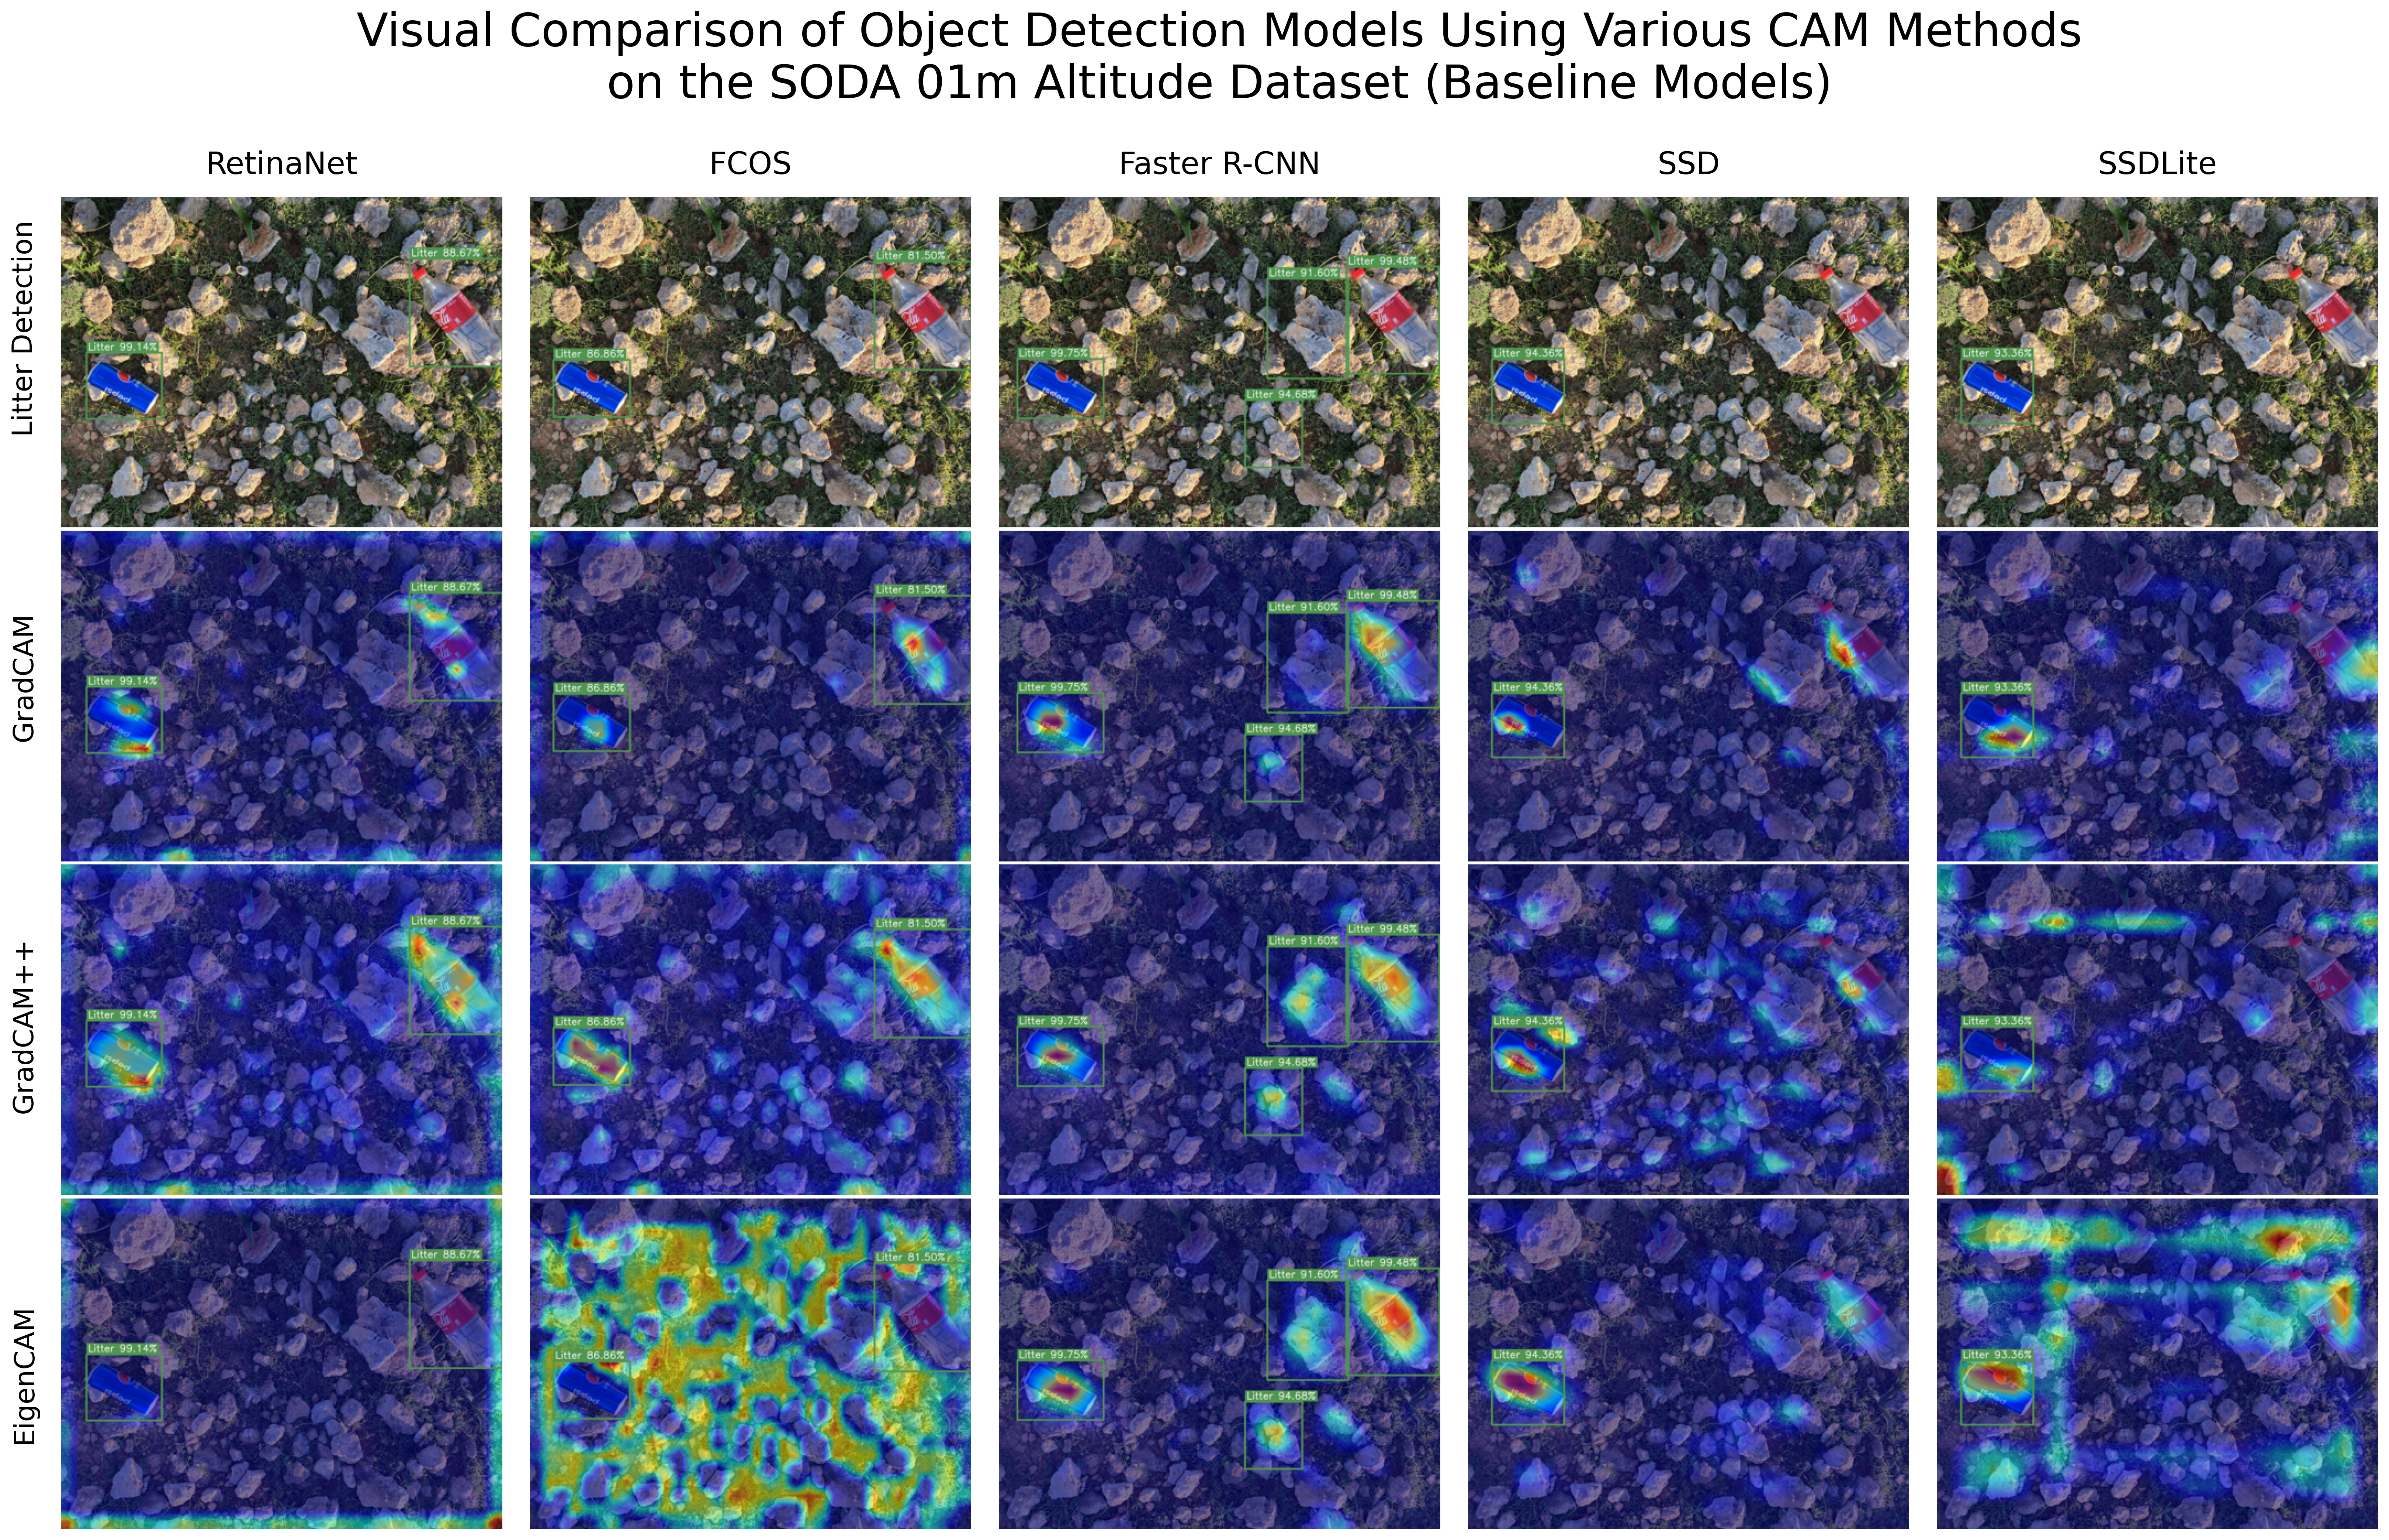
\includegraphics[width=1\textwidth]{gradcam_comparison_baseline.png}
%     \caption{Visual comparison of baseline object detection models using various \gls{cam} methods on the \gls{soda} dataset at a 1-metre altitude for binary litter detection.}
%     \label{fig:gradcam_baseline}
% \end{figure}

% \begin{figure}[!ht]
%     \centering
%     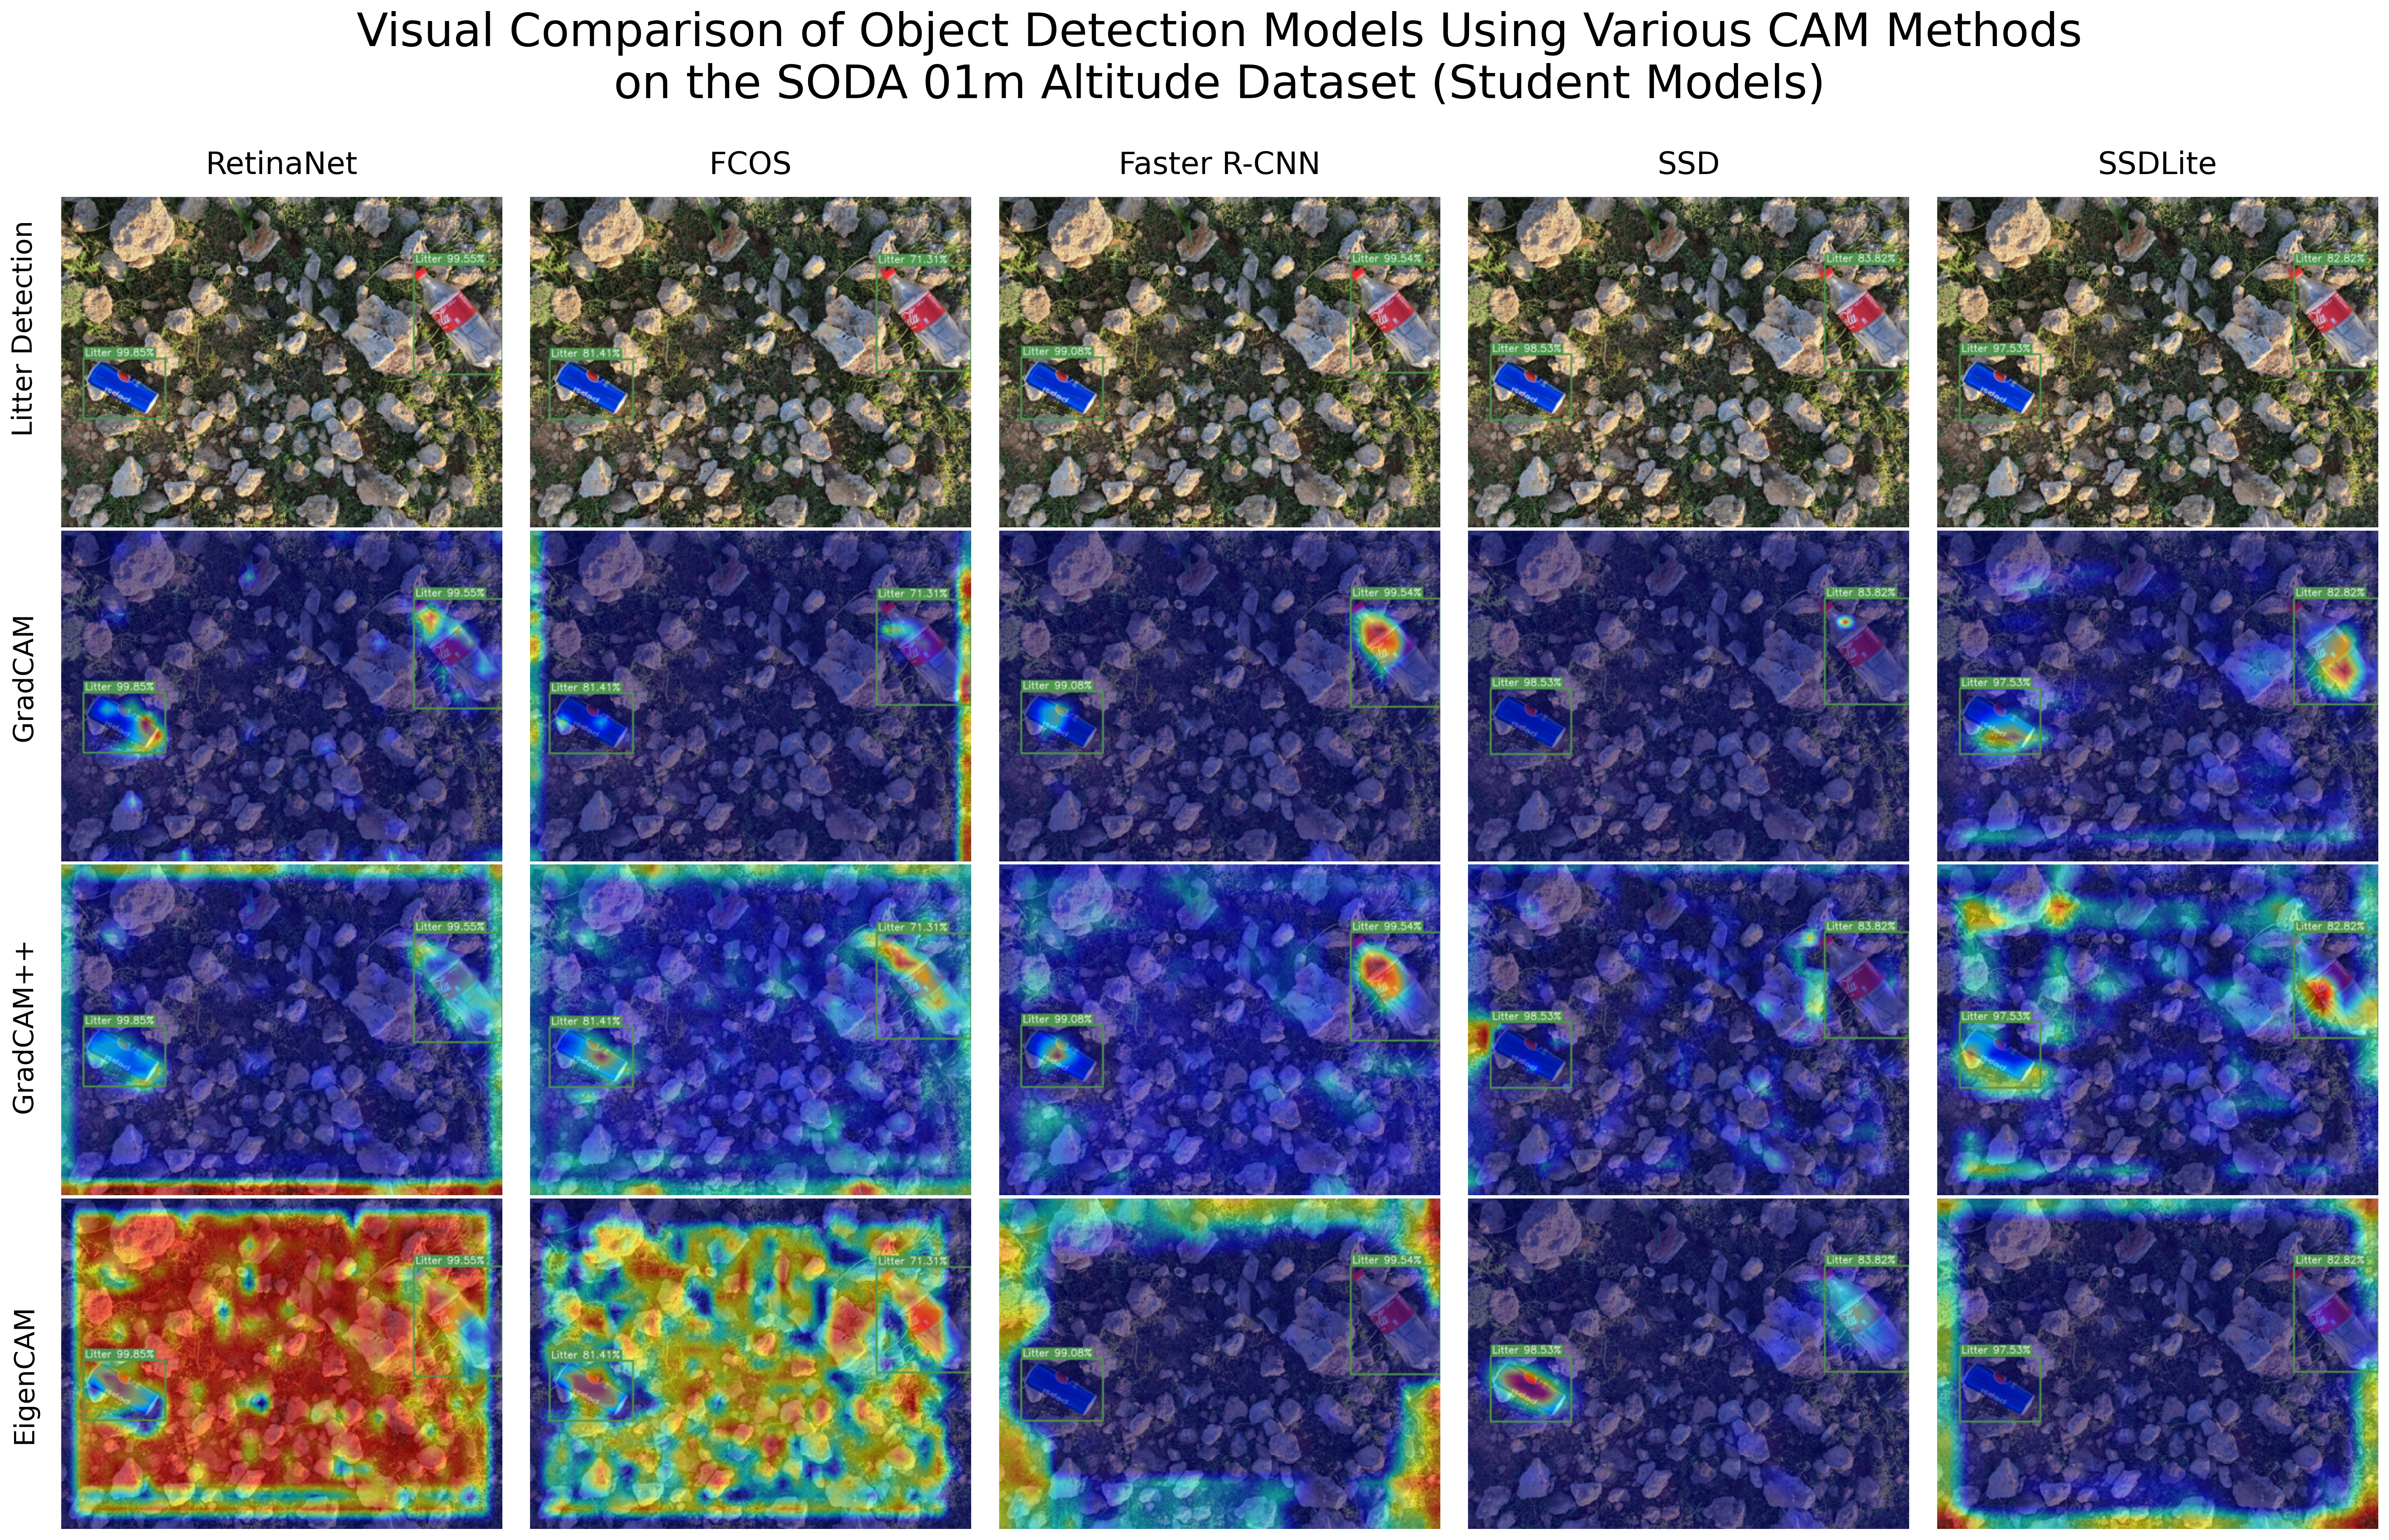
\includegraphics[width=1\textwidth]{gradcam_comparison_student.png}
%     \caption{Visual comparison of student object detection models using various \gls{cam} methods on the \gls{soda} dataset at a 1-metre altitude for binary litter detection.}
%     \label{fig:gradcam_student}
% \end{figure}

\section{Failure Cases in Privileged Information Generation}
\label{sec:5_fail_cases_priv_info_gen}

% One showing overlapping objects of the same time the other object occlusion which is mitigated through sorting

% \begin{figure}[ht]
%   \centering
%   \begin{tabular}{cc}
%     \includegraphics[width=0.48\textwidth]{fail_case1.jpg} &
%     \includegraphics[width=0.48\textwidth]{fail_case2.jpg} \\
%     \small (a) & \small (b) \\
%     \addlinespace[1em]
%     \includegraphics[width=0.48\textwidth]{fail_case3.jpg} &
%     \includegraphics[width=0.48\textwidth]{fail_case4.jpg} \\
%     \small (c) & \small (d) \\
%   \end{tabular}
%   \caption{Showcasing failure cases related to privileged information generation. (a) and (c) are original images from the Pascal VOC 2012 dataset, while (b) and (d) represent the corresponding privileged information.}
%   \label{fig:fail_cases}
% \end{figure}

\section{Discussion}
\label{sec:5_discussion}
Mention total number of models trained and number evaluated an consider mentioning in abstract

\section{Conclusion}
\label{sec:5_conclusion}



%--

\begin{itemize}
    \item UREC Ethics Form - Done
    \item Problem Definition
    \item pages 110-120 maximum
    \item To check Daniel thesis
\end{itemize}

Evaluation
\begin{itemize}
    \item Tiling experiment - SODA include and exclude one meter magnification for SODA - Done

    \item Experiment 1 - Within dataset evaluation
    \item Within dataset - 3 tas SODA Dataset - show all charts and tables + discussion
    \item Ablation studies - alpha for LUPI and Distillation (nest inside)
    \item Across dataset - BDW and UAVVaste
    \item Generalisation - Pascal VOC
    \item Visual Analysis, Ground truth, mask overlap, litter predictions
    \item Interpretability Grad CAM
    \item Discussion - Go over research question once more, theoretical aspect, Knowledge Distillation and Applications - Project AWIGS, summary
\end{itemize}

Conclusion
Revisting aims and objectives
limitation and future work (everything from future work goes here)
Conclusion

Future Work - Future Research/Future Projects
\begin{itemize}
    \item Trying out this method for Segmentation
    \item generalisation capabilities on Pascal VOC and COCO to ask what to include
    \item Test out the method on state-of-the art object deteciton architectures such as YOLO11 etc. . . - can be a limitation
    \item considerations of real time or alternatives to privileged information
    \item Improvement in terms of encoding the bounding boxes for the teacher better and iinvestigating in better channels etc. . . (to ask)
    \item further tests on generalisation of higher class datasets and training parameters
\end{itemize}

%--
